\documentclass[conference]{IEEEtran}

\usepackage[T1]{fontenc}
\usepackage[utf8]{inputenc}
\usepackage{graphicx}
\usepackage{amsmath}
\usepackage{booktabs}
\usepackage{url}
\usepackage{xcolor}

\title{Image-to-Image Translation from Semantic Label Maps with Pix2Pix on Cityscapes}

\author{
\IEEEauthorblockN{Santiago Delgado Ferreiro and David Carballo Rodriguez}
\IEEEauthorblockA{Master in Artificial Intelligence\\
Computer Vision II}
}

\begin{document}

\maketitle

\begin{abstract}
This project addresses paired image-to-image translation from semantic label maps to realistic urban scenes using the Cityscapes subset assigned in the Computer Vision II course. A baseline Pix2Pix model was implemented with a U-Net generator, a PatchGAN discriminator, adversarial supervision, and an $L_1$ reconstruction term. A second model was then designed to improve perceptual quality through paired data augmentation, a least-squares adversarial objective, and residual bottleneck blocks in the generator. Both models were trained and evaluated on a fixed train/validation/test split of 350/75/75 images. On the test set, the improved model obtained a lower mean absolute error and a higher structural similarity index than the baseline, while keeping a comparable PSNR. The repository also includes trained weights for demo inference and a command-line program for paired-sample or standalone label-map generation.
\end{abstract}

\section{Introduction}
Image-to-image translation aims to learn a mapping between two visual domains while preserving the spatial structure shared by both representations. In the paired setting, each source image has a target counterpart that describes the desired output. Pix2Pix~\cite{isola2017pix2pix} is a standard solution for this problem because it combines a conditional adversarial objective with a reconstruction loss, encouraging realism and fidelity at the same time.

In this project, the goal is to translate semantic label maps into realistic RGB street scenes. The assigned dataset is a 500-image Cityscapes subset where every sample concatenates a real image on the left half and its semantic label map on the right half. This formulation is relevant because realistic synthesis from symbolic scene descriptions can support simulation, data generation, and rapid prototyping of downstream perception systems.

The objectives of the work are threefold: first, to implement a correct and reproducible Pix2Pix baseline; second, to propose a small but justified improvement over the baseline; and third, to provide an inference demo that can be executed independently from the training code. The full implementation is available in the accompanying repository. The public repository URL is: \url{https://github.com/santidelgadof/proyecto_final_2_david}.

\section{Technical Approach}
\subsection{Dataset and preprocessing}
The dataset contains 500 paired JPEG images with a spatial resolution of $512 \times 256$, where each half has size $256 \times 256$. During loading, every sample is split into a target RGB image and a conditioning label map. A fixed random seed of 42 was used to build a reproducible split with 350 training images, 75 validation images, and 75 test images.

All inputs were resized to $256 \times 256$ and normalized to $[-1,1]$. The baseline model uses only this deterministic preprocessing. The improved model additionally applies paired data augmentation in the training split: horizontal flipping and resize-crop augmentation with a 16-pixel margin. The same random transformation is always applied to both the label map and the RGB target in order to preserve alignment.

\subsection{Baseline Pix2Pix}
The baseline follows the original Pix2Pix design~\cite{isola2017pix2pix}. The generator is a U-Net with encoder-decoder structure and skip connections that propagate spatial details from early feature maps to late decoding stages. The discriminator is a PatchGAN classifier that receives the concatenation of the conditioning label map and either the real image or the generated one, and predicts realism at the patch level.

The baseline optimization objective combines adversarial supervision and pixel-wise reconstruction:
\begin{equation}
\mathcal{L}_{G}=\mathcal{L}_{GAN}(G,D)+\lambda\mathcal{L}_{1}(G),
\end{equation}
where $\lambda=100$. Binary cross-entropy with logits is used for the adversarial term and the Adam optimizer is configured with learning rate $2\times10^{-4}$ and $\beta_1=0.5$ for both networks.

\subsection{Improved model}
The second model modifies the baseline in three controlled ways. First, the generator bottleneck includes two residual blocks, which increase representational capacity while preserving the overall U-Net structure. Second, the adversarial loss is replaced by the least-squares GAN objective, which is often more stable and encourages smoother gradients. Third, paired augmentation is enabled in the training split to reduce overfitting to the limited dataset size.

These changes were selected because they have a direct implementation cost that is low enough for a course project while still being technically meaningful. The comparison remains fair because both models use the same split, optimizer family, image size, and $L_1$ weight.

\subsection{Training and demo}
Both experiments were trained in Python with PyTorch on a CUDA-enabled GPU using mixed precision. Given the time budget for this deliverable, both configurations were trained for 3 epochs with batch size 4. The repository contains summary files and qualitative previews for both experiments, plus an inference-ready checkpoint for the demo. In addition, a standalone demo script receives an input image and trained weights and writes the synthesized RGB output to disk.

\section{Results}
Table~\ref{tab:results} summarizes the quantitative comparison on the held-out test set. Three metrics were measured: mean absolute error (MAE), peak signal-to-noise ratio (PSNR), and structural similarity index (SSIM). Lower MAE is better, while higher PSNR and SSIM indicate higher fidelity.

\begin{table}[t]
\caption{Test-set comparison between the baseline and the improved model.}
\label{tab:results}
\centering
\begin{tabular}{lccc}
\toprule
Model & MAE $\downarrow$ & PSNR $\uparrow$ & SSIM $\uparrow$ \\
\midrule
Baseline Pix2Pix & 0.2006 & 17.0483 & 0.6023 \\
Improved model & 0.1982 & 17.0078 & 0.6100 \\
\bottomrule
\end{tabular}
\end{table}

The improved configuration achieved the best MAE and SSIM, indicating that it reconstructs the target images slightly more accurately while also preserving scene structure better. PSNR is marginally lower, but the difference is negligible relative to the gain in SSIM. Validation curves also show that the improved model catches up after a weaker first epoch and then surpasses the baseline in structural similarity by epoch 3.

Figure~\ref{fig:qualitative} presents a qualitative example. Both models recover the coarse road layout, skyline, and object silhouettes, which confirms that the conditional mapping has been learned correctly. However, the outputs remain blurred and low-frequency, especially for thin structures and texture-rich regions. This behavior is expected with short training schedules and strong reliance on pixel-wise reconstruction.

\begin{figure}[t]
\centering
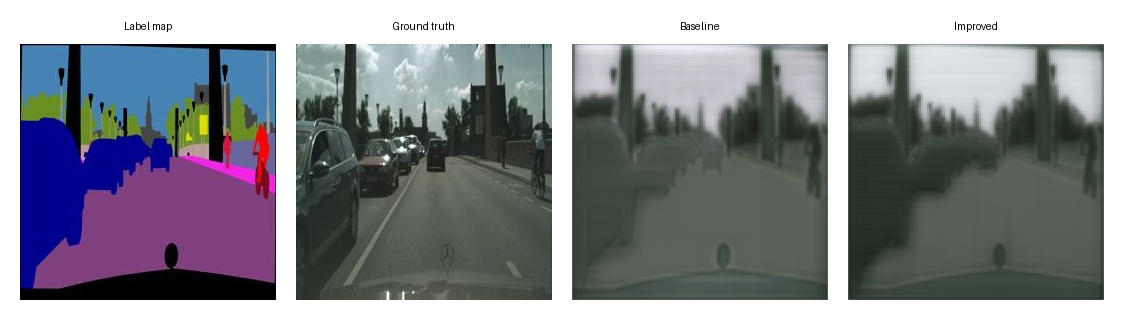
\includegraphics[width=\linewidth]{figures/qualitative_comparison.png}
\caption{Qualitative comparison on one Cityscapes sample. From left to right: label map, ground-truth image, baseline prediction, and improved prediction.}
\label{fig:qualitative}
\end{figure}

From an engineering perspective, the project requirements were completed: the baseline model was implemented, at least one improvement was proposed and evaluated, performance metrics were computed, and a demo program was delivered together with trained inference weights. The experiment is fully reproducible from the configuration files saved in the repository.

\section{Conclusion}
This work implemented a complete Pix2Pix pipeline for semantic-label-to-image translation on the Cityscapes subset assigned in the course. The baseline reproduced the expected conditional GAN behavior and produced coherent scene layouts from label maps. The proposed improvement, based on residual bottleneck blocks, LSGAN loss, and paired augmentation, yielded a measurable gain in MAE and SSIM without increasing system complexity excessively.

The main limitation of the current experiments is the short training schedule. Additional epochs, learning-rate scheduling, and stronger perceptual losses are natural next steps and would likely improve visual sharpness. Even so, the present system already satisfies the assignment goals and provides a solid, well-documented foundation for further experimentation.

\bibliographystyle{IEEEtran}
\bibliography{references}

\end{document}
